\begin{appendices}

%Some Table of Contents entry formatting
\addtocontents{toc}{\protect\renewcommand{\protect\cftchappresnum}{\appendixname\space}}
\addtocontents{toc}{\protect\renewcommand{\protect\cftchapnumwidth}{6em}}

%Begin individual appendices, separated as chapters

\chapter{Supporting Information for chapter 4}


\section{Equations of motion}

As described in the main text, we consider a particle at location $\ve{x}_p=[x_p,y_p]$ with orientation $\theta$ moving with a linear velocity $\ve{U}$ and angular velocity $\Omega$.  The components of the linear velocity in the particle frame are parameterized as $\ve{U}=[U \cos\alpha, U\sin \alpha]$, where $U$ is the linear speed and the angle $\alpha$ describes the direction of motion in the particle frame.  The resulting particle dynamics are given by
\begin{align}
    \dot{\theta} &= \Omega \label{eq:theta}
    \\ 
    \dot{x}_p &= U \cos(\theta + \alpha) \label{eq:xp} 
    \\ 
    \dot{y}_p &= U \sin(\theta + \alpha)\label{eq:yp}
\end{align}	
The velocity parameters $U$, $\alpha$, and $\Omega$ are assumed to depend on the value of a scalar stimulus field $S(\ve{x},t)$ evaluated at the particle center---for example, $\alpha=\alpha(S(\ve{x}_p,t))$. Here, we consider the specific case of a uniform stimulus gradient in the $x$-direction such that $S(\ve{x})= G x$, where $G$ is the gradient magnitude. Dividing equations (\ref{eq:xp}) and (\ref{eq:yp}) by equation (\ref{eq:theta}), we can write the dynamics for the particle position in terms of its orientation $\theta$ 
\begin{align}
    \frac{d x_p}{d\theta} &= R \cos(\theta + \alpha) \label{eq:xp2} 
    \\ 
    \frac{d y_p}{d\theta} &= R \sin(\theta + \alpha)\label{eq:yp2}
\end{align}	
where $R=\Omega/U$ is the radius of curvature of the particle trajectory (in the particle frame). 

%%%%%%%%%%%%%%%%%%%%%%%%%%%%%%%%%%%%%%%%%
%%%%%%%%%%%%%%%%%%%%%%%%%%%%%%%%%%%%%%%%%
\subsection{Approximate solution for weak gradients}

In the absence of a stimulus gradient ($G=0$), equations(\ref{eq:xp2}) and (\ref{eq:yp2}) describe a simple circular orbit of radius $R$
\begin{align}
    x_p(\theta) = C_1 + R \sin(\theta + \alpha) \label{eq:xp3} 
    \\
    y_p(\theta) = C_2 - R \cos(\theta + \alpha)\label{eq:yp3} 
\end{align}
where $C_1$ and $C_2$ are constants that describe the position of the particle at some initial orientation.  In a weak gradient ($G\neq 0$), the radius $R$ and phase $\alpha$ of the particle's circular motion are expected to evolve slowly in time.  To obtain the slow dynamics, we use a two-timing perturbation technique\autocite{Strogatz2015} that distinguishes a fast variable $\tau=\theta$ and a slow variable $T=\varepsilon \theta$ where $\varepsilon$ is a small parameter proportional to the gradient magnitude $G$. The particle position is then expanded as
\begin{equation}
    \ve{x}_p(\theta,\varepsilon) = \ve{x}_0(\tau,T) + \varepsilon \ve{x}_1(\tau,T) + O(\varepsilon^2)
\end{equation}
We substitute this expansion into equations (\ref{eq:xp2}) and (\ref{eq:yp2}) and collect like powers of $\varepsilon$. At zeroth order in $\varepsilon$, the solution is equivalent to equations (\ref{eq:xp3}) and (\ref{eq:yp3}) above. At first order in $\varepsilon$, the governing equations become
\begin{align}
    \partial_T x_0 + \partial_{\tau} x_1 = G x_0 \left[ R' \cos(\tau + \alpha) - R \alpha' \sin(\tau + \alpha)\right] \label{eq:xp4} 
    \\
    \partial_T y_0 + \partial_{\tau} y_1 = G x_0 \left[ R' \sin(\tau + \alpha) + R \alpha' \cos(\tau + \alpha)\right] \label{eq:yp4}
\end{align}
Averaging over the fast variable $\tau$ from 0 to $2\pi$, we obtain the following expressions for the drift velocity in the stimulus gradient    
\begin{align}
    \langle \partial_{\tau} x_1 \rangle &=  - \tfrac{1}{2} G R^2\alpha' \label{eq:drift}
    \\
    \langle \partial_{\tau} y_1 \rangle &= \tfrac{1}{2} G R R' \label{eq:drift2}
\end{align}
where the prime denotes differentiation with respective to the slow variable. To avoid net motion of the particle in the $y$ direction, the radius of the trajectory $R$ must be independent of the stimulus such that $R'=0$.  Equation (\ref{eq:drift}) provides an estimate of the drift velocity in the $x$-direction due to the changing orientation of the particle velocity in the stimulus landscape.  The accuracy of this approximation requires that drift velocity be slow relative to the circular motion of the particle, which implies that $G R\alpha' \ll 1$.  Figure \ref{fig:SimpleModel} highlights the performance of this analytical approximation for a specific response function $\alpha(S)$.
\begin{figure}[h]
    \centering
    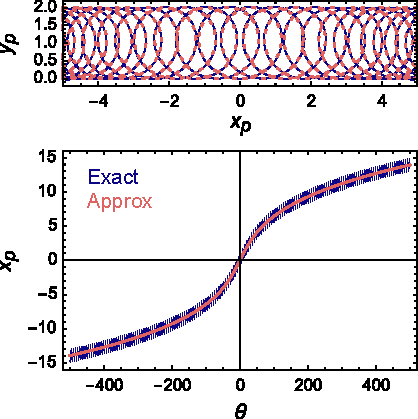
\includegraphics[width=9cm]{figures/A3_SimpleModel.pdf}
    \caption{Computed particle trajectory for $\alpha(S) = \arctan(-0.2 S)$ and $R=\text{constant}$ in a uniform stimulus gradient $S=G x$. Here, lengths are scaled by the curvature radius $R$ and stimuli by $GR$ (corresponding to $R\rightarrow1$ and $G\rightarrow1$). The solid purple curve shows the exact result; the dashed pink curve shows the slow dynamics described by equation (\ref{eq:drift}). The small parameter governing the accuracy of the approximation is $G R\alpha' = 0.2 \ll 1$.}
    \label{fig:SimpleModel}
\end{figure}


%%%%%%%%%%%%%%%%%%%%%%%%%%%%%%%%%%%%%%%%%
%%%%%%%%%%%%%%%%%%%%%%%%%%%%%%%%%%%%%%%%%
\subsection{Choice of sensor location}

The particle's velocity is assumed to depend on the stimulus magnitude evaluated at the particle center $\ve{x}_p$.  If the stimulus magnitude is instead evaluated at a different position on the particle $\ve{x}_s\neq \ve{x}_p$, the resulting dynamics will be slightly different.  However, such differences are negligible when the characteristic size of the particle is much smaller than the radius of its periodic orbit.  To show this, we consider how the drift velocity depends on the sensor position $\ve{x}_s$, at which the stimulus is ``sensed'' by the particle.  We assume that the particle has fixed response functions $R(S)$ and $\alpha(S)$ where $S = S(\ve{x}_s(t))$. In the particle frame, we defined the constant displacement between the sensor and the particle center as $\ve{x}_s-\ve{x}_p =[\delta \cos\beta, \delta \sin\beta]$.  The dynamics of equations (\ref{eq:xp2}) and (\ref{eq:yp2}) are modified as
\begin{align}
    \frac{d x_p}{d\theta} &= R(G x_s ) \cos(\theta + \alpha(G x_s))   
    \\ 
    \frac{d y_p}{d\theta} &= R(G x_s) \sin(\theta + \alpha(G x_s))
\end{align}	
where $x_s = x_p + \delta  \cos( \theta +\beta)$.  Following the same two-timing scheme described above, the first order equations (\ref{eq:xp4}) and (\ref{eq:yp4}) become
\begin{align}
    \partial_T x_0 + \partial_{\tau} x_1 = G \left[ x_0 + \delta \cos(\tau +\beta)\right] \left[ R' \cos(\tau + \alpha) - R \alpha' \sin(\tau + \alpha)\right]
    \\
    \partial_T y_0 + \partial_{\tau} y_1 = G \left[ x_0 + \delta \cos(\tau +\beta)\right] \left[ R' \sin(\tau + \alpha) + R \alpha' \cos(\tau + \alpha)\right]
\end{align}
Averaging over the fast variable $\tau$ from 0 to $2\pi$, we obtain the following expressions for the drift velocity in the stimulus gradient    
\begin{align}
    \langle \partial_{\tau} x_1 \rangle &= -\tfrac{1}{2} G R^2\alpha' \left( 1 + \frac{\delta}{R}\sin(\alpha-\beta) \right) + \tfrac{1}{2} G R R' \left( \frac{\delta}{R} \cos(\alpha-\beta) \right) \label{eq:xdrift2}
    \\
    \langle \partial_{\tau} y_1 \rangle &= \tfrac{1}{2} G R^2\alpha' \left( \frac{\delta}{R} \cos(\alpha-\beta) \right) + \tfrac{1}{2} G R R'\left( 1 + \frac{\delta}{R}\sin(\alpha-\beta) \right) \label{eq:ydrift2}
\end{align}
Changes in the location of the sensor give rise to corrections in the drift velocity of order $\delta/R$ relative to equations (\ref{eq:drift}) and (\ref{eq:drift2}).  Figure \ref{fig:SensorLocation} shows two computed particle trajectories with $\delta=0$ and $\delta = 0.1 R$ to illustrate the effect of sensor location on particle chemotaxis.
\section{Model details for rigid self-phoretic clusters}

We consider the self-phoretic propulsion of a rigid cluster of $N$ solid spheres of radii $a_j$. Each sphere $j$ releases a constant flux $A_j$ of a solute from its surface $\mathcal{S}_j$  
\begin{equation}
    -D \ve{n}\cdot \nabla c(\ve{x}) = A_j \quad \text{for} \quad \ve{x} \in \mathcal{S}_j \label{eq:bc1}
\end{equation}
where $D$ is the diffusivity, and $\ve{n}$ is the unit normal vector directed out from the surface.  The solute concentration $c(\ve{x})$ around the spheres quickly approaches a steady-state distribution governed by the Laplace equation
\begin{equation}
    \nabla^2 c = 0
\end{equation}
Far from the particle cluster, the solute concentration approaches a constant value $c^{\infty}$, which can be set to zero without loss of generality. 

The solute gradients generated by the particles produce a phoretic slip velocity tangent to the surface of each sphere 
\begin{equation}
    \ve{u}_s(\ve{x}) = \mu_j (\ve{I}-\ve{n}\ve{n}) \cdot \nabla c(\ve{x}) 
\end{equation}
where $\mu_j$ is the phoretic mobility of sphere $j$, and $\ve{I}$ is the identity tensor. At small Reynolds numbers, the fluid velocity $\ve{u}(\ve{x})$ surrounding the particle is governed by the Stokes equations
\begin{equation}
    0 = -\nabla p + \eta \nabla^2 \ve{u} \quad \text{and}\quad \nabla\cdot\ve{u} = 0
\end{equation}
where $\eta$ is the fluid viscosity.  The cluster of spheres moves as a rigid body with linear velocity $\ve{U}$ and angular velocity $\ve{\Omega}$.  At the surface of each sphere $j$, the fluid velocity is equal to that of the sphere plus the slip velocity  
\begin{equation}
    \ve{u}(\ve{x}) = \ve{U} + \ve{\Omega}\times(\ve{x}_j - \ve{x}_p) + \ve{u}_s(\ve{x}) \quad \text{for} \quad \ve{x} \in \mathcal{S}_j
\end{equation}
where $\ve{x}_p$ denotes the center of the composite particle.  Far from the particle, the fluid is stationary.  Finally, the velocities $\ve{U}$ and $\ve{\Omega}$ are determined by the condition that the net force and torque on the particle vanish
\begin{equation}
    0 = \int_{\mathcal{S}} (\ve{\sigma}\cdot\ve{n}) \mathrm{d}\mathcal{S}  \quad \text{and} \quad 0 = \int_{\mathcal{S}} (\ve{x}-\ve{x}_p)\times (\ve{\sigma}\cdot\ve{n} )\mathrm{d}\mathcal{S}  \label{eq:noForceTorque}
\end{equation}
where $\ve{\sigma} = -\nabla p + \eta(\nabla\ve{u}+\nabla\ve{u}^T)$ is the stress tensor.

%%%%%%%
%%%%%%%%   
%%%%%%%%
%%%%%%%%%%
%%%%%%%%%%
%%%%%%%%%%%
%%%%%%%%%%
%%%%%%%%%%
%%%%%%%%%%
%%%%%%%
%%%%%%%%
%%%%%%%%
%%%%%%%%%%
%%%%%%%%%%
%%%%%%%%%%%
%%%%%%%%%%
%%%%%%%%%%
%%%%%%%%%%
%%%%%%%
%%%%%%%%
%%%%%%%%
%%%%%%%%%%
%%%%%%%%%%
%%%%%%%%%%%
%%%%%%%%%%
%%%%%%%%%%
%%%%%%%%%%
\subsection{Diffusion Problem}

To approximate the solution to the diffusion problem, we start from the following integral solution for the concentration field
\begin{equation}
    c(\ve{x}) - c^{\infty}(\ve{x}) = \int_{\mathcal{S}} \left\{ c(\ve{y})[\ve{n}(\ve{y})\cdot \nabla_y G(\ve{y},\ve{x})]  -  G(\ve{y},\ve{x}) [\ve{n}(\ve{y})\cdot \nabla c(\ve{y})] \right\} d \mathcal{S}(\ve{y})
\end{equation}
where $\ve{n}$ is the unit normal vector directed into the fluid, and $G(\ve{y},\ve{x})$ is the Green's function for the concentration at $\ve{y}$ due to a point source at $\ve{x}$.  Expanding the Green's function in a Taylor series in $\ve{y}$ about the center $\ve{x}_j$ of each sphere $j$, we obtain
\begin{equation}
    c(\ve{x}) - c^{\infty}(\ve{x})  = \sum^N_{j=1} \left[ C_0^j G(\ve{x}_j,\ve{x}) + \ve{C}_1^j\cdot \nabla_y G(\ve{y},\ve{x})\rvert_{\ve{y}=\ve{x}_j} + \dots \right] 
\end{equation}
where the first and second moments are 
\begin{gather}
    C_0^j = \int_{\mathcal{S}_j} - \ve{n}(\ve{y})\cdot \nabla c(\ve{y})d \mathcal{S}(\ve{y})
    \\
    \ve{C}_1^j = \int_{\mathcal{S}_j} \left\{ c(\ve{y})\ve{n}(\ve{y}) - (\ve{y}-\ve{x}_j)[\ve{n}(\ve{y})\cdot \nabla c(\ve{y})] \right\} d \mathcal{S}(\ve{y})
\end{gather}
We have truncated this multipole expansion at the dipole level; however, higher order contributions can be derived in a similar manner. Substituting the boundary condition (\ref{eq:bc1}) for the surface flux, the above moments can be simplified as
\begin{gather}
    C_0^j = \frac{4\pi a_j^2 A_j}{D}
    \\
    \ve{C}_1^j = \int_{\mathcal{S}_i} c(\ve{y})\ve{n}(\ve{y}) d \mathcal{S}(\ve{y})
\end{gather}
In an unbounded domain, the Green's function is $G(\ve{y},\ve{x}) = (4\pi \lvert \ve{y}-\ve{x}\rvert)^{-1}$, and the multipole expansion for the concentration becomes
\begin{equation}
    c(\ve{x}) - c^{\infty}(\ve{x})  = \frac{1}{4\pi} \sum^N_{j=1} \left[ \frac{C_0^j}{\lvert\ve{x}-\ve{x}_j\rvert}  + \frac{\ve{C}_1^j\cdot(\ve{x}-\ve{x}_j)}{\lvert\ve{x}-\ve{x}_j\rvert^3} + \dots \right] \label{eq:multipole}
\end{equation}

To solve for the dipole moments $\ve{C}_1$, we make used of the following relations (so-called Fax\'en laws\autocite{Bonnecaze1990,OBrien1979}) for a sphere $i$ in an external concentration field $c'(\ve{x})$ 
\begin{gather}
    c(\ve{x}_i) - c'(\ve{x}_i) = \frac{C_0^i}{4\pi a_i}  \label{eq:faxen1}
    \\
    -\nabla c'(\ve{x}_i) = \frac{\ve{C}_1^i}{2\pi a_i^3}  \label{eq:faxen2}
\end{gather}
Here, the external concentration and its gradient are evaluated at the center of the sphere in its absence; the particle concentration $c(\ve{x}_i)$ is defined as the average concentration on the surface of the sphere
\begin{equation}
    c(\ve{x}_i) \equiv \frac{1}{4\pi a_i^2} \int_{\mathcal{S}_i} c(\ve{x}) d\mathcal{S}(\ve{x}) 
\end{equation}
Combing the Fax\'en laws (\ref{eq:faxen1}) and (\ref{eq:faxen2}) with the multipole expansion (\ref{eq:multipole}), we obtain the following linear equations
\begin{equation}
    \begin{bmatrix} c_i-c^{\infty}_i \\ c_j-c^{\infty}_j \\ \vdots \\ -\nabla c^{\infty}_i \\ -\nabla c^{\infty}_j \\ \vdots \end{bmatrix} = 
    \begin{bmatrix} 
        a_{ii} & a_{ij} & \cdots &\ve{\tilde{b}}_{ii} & \ve{\tilde{b}}_{ij} & \cdots \\
        a_{ji} & a_{jj} & \cdots & \ve{\tilde{b}}_{ji} & \ve{\tilde{b}}_{jj} & \cdots \\
        \vdots & \vdots & & \vdots & \vdots &  \\
        \ve{b}_{ii} & \ve{b}_{ij} & \cdots & \ve{c}_{ii} & \ve{c}_{ij} & \cdots \\
        \ve{b}_{ji} & \ve{b}_{jj} & \cdots & \ve{c}_{ji} & \ve{c}_{jj} & \cdots \\
        \vdots & \vdots & & \vdots & \vdots &  \\
    \end{bmatrix}
    \cdot
    \begin{bmatrix} C^i_0 \\ C^j_0 \\ \vdots \\ \ve{C}^i_1 \\ \ve{C}^j_1 \\ \vdots \end{bmatrix} \label{eq:grandPotential}
\end{equation}
where $c_i=c(\ve{x}_i)$ and $\nabla c^{\infty}_i=\nabla c^{\infty}(\ve{x}_i)$.  The quantities $a$, $\ve{\tilde{b}}$, $\ve{b}$, and $\ve{c}$ are components of the grand potential tensor (so-called in electrostatics\autocite{Bonnecaze1990})
\begin{gather}
    a_{ii} = \frac{1}{4\pi a_i} \quad \text{and} \quad  a_{ij} = a_{ji} = \frac{1}{4\pi r_{ij}}
    \\
    \ve{\tilde{b}}_{ii} = \ve{b}_{ii} = 0 \quad \text{and} \quad \ve{\tilde{b}}_{ij} = -\ve{\tilde{b}}_{ji} = -\ve{b}_{ij} = \ve{b}_{ji} = \frac{\ve{\hat{r}}_{ij}}{4\pi r_{ij}^2} 
    \\
    \ve{c}_{ii} = \frac{\ve{I}}{2\pi a_i^3} \quad \text{and} \quad \ve{c}_{ij} = \ve{c}_{ji} =  \frac{1}{4\pi r_{ij}^3} \left(\ve{I} - 3\ve{\hat{r}}_{ij}\ve{\hat{r}}_{ij}\right)
\end{gather}
with $\ve{r}_{ij} = \ve{x}_i - \ve{x}_j$ and $\ve{\hat{r}}_{ij} = \ve{r}_{ij}/ r_{ij}$.  In the present context, the external concentration field is absent (i.e., $c^{\infty}(\ve{x})=0$) and the monopole moments $C_0$ are known.  We can therefore solve equation (\ref{eq:grandPotential}) for the unknown dipole moments $\ve{C}_1$.  This approach is equivalent to the method of reflections detailed by Michelin \emph{et al.}\autocite{varma2018clustering}  The magnitude of dipole moment  scales as $C_1^j \propto (a/d)^2$ where $a$ is a typical sphere radius and $d$ is a characteristic separation between spheres. Truncating the multipole expansion at the dipole level introduces errors of order $(a/d)^7$ in estimating the dipole moments $\ve{C}_1^j$.    

%%%%%%%%%%%%%%%%%%%%%%%%%%%%%%%%%%%%%%%%%
%%%%%%%%%%%%%%%%%%%%%%%%%%%%%%%%%%%%%%%%%
\subsection{Hydrodynamic Problem}

Owing to the linearity of the Stokes equations, the stress tensor $\ve{\sigma}$ can be decomposed as the sum of two parts: first that of the moving spheres with no slip at their surface (denoted $\ve{\sigma}'$), and second that of stationary spheres with a prescribed slip velocity at their surface (denoted $\ve{\sigma}''$).  The no force and torque conditions (\ref{eq:noForceTorque}) can then be written as
\begin{gather}
    0 = \sum_j \ve{F}'_j +  \int_{\mathcal{S}} (\ve{\sigma}''\cdot\ve{n}) \mathrm{d}\mathcal{S} \label{eq:noForce}
    \\
    0 = \sum_j \left[(\ve{x}_j-\ve{x}_p)\times \ve{F}'_j + \ve{L}'_j\right] +  \int_{\mathcal{S}} (\ve{x}-\ve{x}_p)\times(\ve{\sigma}''\cdot\ve{n}) \mathrm{d}\mathcal{S}   \label{eq:noTorque}
\end{gather}
where $\ve{F}'_j$ and $\ve{L}'_j$ are the hydrodynamic drag force and torque on sphere $j$ due to its motion and that of the neighboring spheres (in the absence of activity). The integrals can be simplified by use of the Lorentz reciprocal theorem,\autocite{Kim2005} which relates the two flows $\ve{u}'$ and $\ve{u}''$ as 
\begin{equation}
    \int_{\mathcal{S}} \ve{u}'\cdot(\ve{\sigma}''\cdot\ve{n})  \mathrm{d}\mathcal{S} =  \int_{\mathcal{S}} \ve{u}''\cdot(\ve{\sigma}'\cdot\ve{n}) \mathrm{d}\mathcal{S} \label{eq:lorentz}
\end{equation}
The velocity $\ve{u'}$ at a point $\ve{x}$ on the surface of the rigid particle is $\ve{u'}=\ve{U}+\ve{\Omega}\times(\ve{x}-\ve{x}_p)$. Additionally, the normal stress on the surface of sphere $j$ is  $\ve{\sigma}'\cdot \ve{n}_j= -\tfrac{3\eta}{2a_j}\ve{U}_j-3\eta\ve{\Omega} \times\ve{n}_j$, where  $\ve{U}_j = \ve{U} +\ve{\Omega}\times(\ve{x}_j-\ve{x}_p)$ is the velocity of sphere $j$, and $\ve{n}_j$ is the unit normal directed out from the sphere.\autocite{Stone1996} Substituting these quantities into equation (\ref{eq:lorentz}) and collecting like terms in $\ve{U}$, we obtain
\begin{equation}
    \int_{\mathcal{S}} (\ve{\sigma}''\cdot\ve{n}) \mathrm{d}\mathcal{S}  = -\sum_j 6\pi\eta a_j \ve{U}_j^A \quad \text{with}\quad \ve{U}_j^A \equiv \frac{1}{4\pi a_j^2}\int_{\mathcal{S}_j} \ve{u}_s\mathrm{d}\mathcal{S} \label{eq:intForce}
\end{equation}
where $\ve{U}^A_j$ is the ``active'' linear velocity of sphere $j$. Similarly, we can collect terms in $\ve{\Omega}$ to obtain
\begin{equation}
    \int_{\mathcal{S}}(\ve{x}-\ve{x}_p)\times(\ve{\sigma}''\cdot\ve{n}) \mathrm{d}\mathcal{S} = -\sum_j\left[  6 \pi \eta a_j (\ve{x}_j-\ve{x}_p)\times\ve{U}^A_j  + 8\pi\eta a_j^3\ve{\Omega}^{A}_j\right] \label{eq:intTorque}
\end{equation}
where the ``active'' angular velocity is 
\begin{equation}
    \ve{\Omega}^{A}_j = \frac{3}{8\pi a_j^4}\int_{\mathcal{S}_j} (\ve{x}-\ve{x}_j) \times \ve{u}_s\mathrm{d}\mathcal{S}
\end{equation}
Substituting equations (\ref{eq:intForce}) and (\ref{eq:intTorque}) into equations (\ref{eq:noForce}) and (\ref{eq:noTorque}), we obtain 
\begin{gather}
    \sum_j \ve{F}'_j  = \sum_j 6\pi \eta a_j \ve{U}^A_j \label{eq:motion1}
    \\
    \sum_j \left[(\ve{x}_j-\ve{x}_p)\times \ve{F}'_j + \ve{L}'_j\right]  = \sum_j  \left(6 \pi \eta a_j (\ve{x}_j-\ve{x}_p)\times\ve{U}^A_j  - 8\pi\eta a_j^3\ve{\Omega}^{A}_j\right) \label{eq:motion2}
\end{gather}

The forces $\ve{F}'_j$ and torques $\ve{L}'_j$ on the solid spheres due to their motion through the fluid (in the absence of activity) are related to the particle velocities $\ve{U}$ and $\ve{\Omega}$ by the hydrodynamic resistance tensor
\begin{equation}
    \begin{bmatrix} \ve{F}'_i \\ \ve{F}'_j \\ \vdots \\ \ve{L}'_i \\ \ve{L}'_j \\ \vdots \end{bmatrix} = 
    \begin{bmatrix} 
        \ve{A}_{ii} & \ve{A}_{ij} & \cdots & \ve{\tilde{B}}_{ii} & \ve{\tilde{B}}_{ij} & \cdots \\ 
        \ve{A}_{ji} & \ve{A}_{jj} & \cdots & \ve{\tilde{B}}_{ji} & \ve{\tilde{B}}_{jj} & \cdots \\  
        \vdots  & \vdots & & \vdots & &  & \\ 
        \ve{B}_{ii} & \ve{B}_{ij} & \cdots & \ve{C}_{ii} & \ve{C}_{ij} & \cdots \\ 
        \ve{B}_{ji} & \ve{B}_{jj} & \cdots & \ve{C}_{ji} & \ve{C}_{jj} & \cdots \\  
        \vdots  & & & \vdots & &  &  
    \end{bmatrix} 
    \cdot
    \begin{bmatrix} \ve{U}_i \\ \ve{U}_j \\ \vdots \\ \ve{\Omega}_i \\ \ve{\Omega}_j \\ \vdots \end{bmatrix}\label{eq:stokes}
\end{equation}
For rigid body motion, the linear and angular velocities of the spheres are related to that of the cluster as $\ve{U}_j=\ve{U}+\ve{\Omega}\times(\ve{x}_j - \ve{x}_p)$ and $\ve{\Omega}_j=\ve{\Omega}$.  Substituting these expressions into equation (\ref{eq:stokes}), we obtain the following relation between the total force and torque on the particle and its linear and angular velocity
\begin{equation}
    \begin{bmatrix} \ve{F}' \\ \ve{L}' \end{bmatrix} = 
    \begin{bmatrix} 
        \ve{A} & \ve{\tilde{B}} \\ 
        \ve{B} & \ve{C} 
    \end{bmatrix} 
    \cdot
    \begin{bmatrix} \ve{U} \\ \ve{\Omega} \end{bmatrix}\label{eq:stokesParticle}
\end{equation}
where the components of the particle resistance tensor are 
\begin{gather}
    \ve{A} = \sum_{i,j} \ve{A}_{ij} \label{eq:A}
    \\
    \ve{\tilde{B}} = \ve{B}^T = \sum_{i,j} \left[(\ve{x}_j -\ve{x}_p) \times \ve{A}_{ij} + \ve{\tilde{B}}_{ij} \right] \label{eq:B}
    \\
    \ve{C} = \sum_{i,j}\left\{(\ve{x}_j -\ve{x}_p) \times [(\ve{x}_j -\ve{x}_p) \times \ve{A}_{ij}] + \ve{C}_{ij}\right\} \label{eq:C}
\end{gather}
Here, the cross products between a vector and a second order tensor indicate $(\ve{a}\times\ve{B})_{mn}=\varepsilon_{mpq} a_p B_{qn}$ where $\varepsilon_{mpq}$ is the alternating unit tensor.  Using the particle resistance tensor, the equations of motion (\ref{eq:motion1}) and (\ref{eq:motion2}) become
\begin{gather}
    \ve{A}\cdot \ve{U} + \ve{\tilde{B}} \cdot \ve{\Omega} = \sum_j 6\pi \eta a_j \ve{U}^A_j
    \\
    \ve{B}\cdot \ve{U} + \ve{C} \cdot \ve{\Omega}  = \sum_j  \left(6 \pi \eta a_j (\ve{x}_j-\ve{x}_p)\times\ve{U}^A_j  - 8\pi\eta a_j^3\ve{\Omega}^{A}_j\right)
\end{gather}

These equations for the particle velocity are exact; we now proceed to make some simplifying approximations to obtain the leading order contributions to the propulsion velocity when the separation between spheres is large relative to their size (i.e., $a/d\ll 1$).

To approximate the resistance tensor, we construct a truncated approximation to the corresponding mobility tensor that includes only the leading order hydrodynamic interactions between the spheres
\begin{equation}
    \begin{bmatrix} \ve{U}_i \\ \ve{U}_j \\ \vdots \\ \ve{\Omega}_i \\ \ve{\Omega}_j \\ \vdots \end{bmatrix}\label{eq:mobility}
    =
    \begin{bmatrix} 
        \ve{a}_{ii} & \ve{a}_{ij} & \cdots & \ve{\tilde{b}}_{ii} & \ve{\tilde{b}}_{ij} & \cdots \\ 
        \ve{a}_{ji} & \ve{a}_{jj} & \cdots & \ve{\tilde{b}}_{ji} & \ve{\tilde{b}}_{jj} & \cdots \\  
        \vdots  & \vdots & & \vdots & &  & \\ 
        \ve{b}_{ii} & \ve{b}_{ij} & \cdots & \ve{c}_{ii} & \ve{c}_{ij} & \cdots \\ 
        \ve{b}_{ji} & \ve{b}_{jj} & \cdots & \ve{c}_{ji} & \ve{c}_{jj} & \cdots \\  
        \vdots  & & & \vdots & &  &  
    \end{bmatrix} 
    \cdot
    \begin{bmatrix} \ve{F}'_i \\ \ve{F}'_j \\ \vdots \\ \ve{L}'_i \\ \ve{L}'_j \\ \vdots \end{bmatrix} 
\end{equation}
Here, the components of the mobility tensor are approximated as 
\begin{gather}
    \ve{a}_{ii} = \frac{1}{6\pi \eta a_i} \quad \text{and} \quad \ve{a}_{ij} = \frac{1}{8\pi \eta r_{ij}} (\ve{I} +\frac{ \ve{\hat{r}}_{ij}\ve{\hat{r}}_{ij}}{r_{ij}^2}    ) + \mathcal{O}(r^{-3}_{ij})
    \\
    \ve{\tilde{b}}_{ii} =\ve{b}_{ii} = 0 \quad \text{and} \quad \ve{\tilde{b}}_{ij} = \ve{b}_{ij} = 0 + \mathcal{O}(r^{-2}_{ij})
    \\
    \ve{c}_{ii} = \frac{1}{8\pi \eta a^3_i} \quad \text{and} \quad \ve{c}_{ij} = 0 + \mathcal{O}(r^{-3}_{ij})
\end{gather}
This truncated approximation to the mobility tensor is evaluated and inverted to obtain the the approximate resistance tensor.  From the diffusion problem above, the active linear velocity can be evaluated as 
\begin{equation}
    \ve{U}_j^A = -\frac{\mu_j \ve{C}_1^j}{2 \pi a_j^3}
\end{equation}
The active angular velocity $\ve{\Omega}_j^A$ depends on the second order moment $\ve{C}_2^j$, which is of order $(a/d)^3$ and neglected in our present analysis.


%%%%%%%%%%%%%%%%%%%%%%%%%%%%%%%%%%%%%%%%%
%%%%%%%%%%%%%%%%%%%%%%%%%%%%%%%%%%%%%%%%%
%%%%%%%%%%%%%%%%%%%%%%%%%%%%%%%%%%%%%%%%%
\clearpage
\section{Definition of standard shapes for shape-shifting particles}

In a shape-shifting cluster, the relative positions and orientations of the spheres are characterized by a single degree of freedom parameterized by $s$. To describe the kinematics of this shape-changing particle, we introduce two coordinate systems: the lab frame $\ve{x}=[x,y,z]$ and the particle frame $\ve{x}'=[x',y',z']$.  If $\ve{v}$ is a vector in the lab frame, then $\ve{v}'=\ve{R}\ve{v}$ is the same vector in the particle frame, where $\ve{R}$ is a rotation matrix that characterizes the relative orientation of the two frames (e.g., specified by the unit quaternion $\ve{q}$).  The position of sphere $j$ in the lab frame is given by 
\begin{equation}
    \ve{x}_j = \ve{x}_p + \ve{R}^T\ve{x}'_j
\end{equation}
where $\ve{x}_p$ is the center of the particle in the lab frame.  The positions of the spheres in the particle frame $\ve{x}'_j$ depend on the shape parameter $s$; the functions $\ve{x}'_j(s)$ define the standard shapes of the composite particle.\autocite{Shapere1989} Upon changes in the shape parameter $s$, the position of sphere $j$ changes as 
\begin{gather}
    \frac{d\ve{x}_j}{d s} = \frac{d \ve{x}_p}{d s} + \frac{d\ve{R}^T}{d s}\ve{x}'_j + \ve{R}^T\frac{d \ve{x}'_j}{ds}
    \\
    \frac{d\ve{x}_j}{d s} = \frac{d \ve{x}_p}{d s} + \frac{d\ve{R}^T}{d s} \ve{R}(\ve{x}_j-\ve{x}_p) + \ve{R}^T\frac{d \ve{x}'_j}{ds}
\end{gather}
The first and second terms describe rigid body translation and rotation through the fluid; the third describes additional motions due to shape change. Importantly, the standard shapes $\ve{x}'_j(s)$ can be defined such that the particle frame does not translate or rotate due to shape change---that is,
\begin{equation}
    \frac{d \ve{x}_p}{d s} = 0 \quad \text{and} \quad \frac{d\ve{R}^T}{d s} = 0
\end{equation}
for all $s$.  Moreover, since $\ve{x}_p$ and $\ve{R}$ are independent of the shape parameter, we are free to choose $\ve{x}_p=0$ and $\ve{R}=\ve{I}$ without loss of generality.  The use of this coordinate system ensures that particle motion is due entirely to phoretic propulsion.

To identify the standard shapes $\ve{x}'_j(s)$,  we start with a third reference frame, in which the positions of the spheres given by known functions $\ve{x}''_j(s)$.  The position and velocity of the sphere $j$ in the lab frame is expressed as 
\begin{gather}
    \ve{x}_j = \ve{x}'_p + \ve{R}'^T \ve{x}''_j 
    \\
    \frac{d\ve{x}_j}{ds} = \frac{d \ve{x}'_p}{ds} + \frac{d\ve{R}'^T}{d s} \ve{R}'(\ve{x}_j-\ve{x}'_p) + \ve{R}'^T\frac{d \ve{x}''_j}{ds} \label{eq:velocity}
\end{gather}
We substitute equation (\ref{eq:velocity}) for the sphere velocity into equation (\ref{eq:stokes}) for the corresponding forces and torques.  Changes in the configuration of the spheres are driven internally such that there is zero net force and torque on the composite particle.  Moreover, we assume that the relative orientations of the spheres do not change during shape-shifting (i.e., $\ve{\Omega}_i=\ve{\Omega}_j$ for all spheres pair $i$ and $j$). With these assumptions, the linear and angular velocity of the particle reference frame ($\ve{x}_p'$ and $\ve{R}'$) are governed by
\begin{gather}
    \ve{A}\ve{U} + \ve{\tilde{B}} \ve{\Omega} = -\sum_{i,j} \ve{A}_{ij} \ve{R}'^T \frac{d \ve{x}_j''}{d s} \label{eq:noForceShape}
    \\
    \ve{B}\ve{U} + \ve{C} \ve{\Omega} = -\sum_{i,j}\left[(\ve{x}_i-\ve{x}_p') \times \ve{A}_{ij} + \ve{B}_{ij}\right] \ve{R}'^T \frac{d \ve{x}_j''}{d s} \label{eq:noTorqueShape}
\end{gather}
where the components of the resistance tensor are given by equations (\ref{eq:A}), (\ref{eq:B}), and (\ref{eq:C}).
Starting from some initial condition $\ve{x}'_p(s_0)=0$ and $\ve{R}'(s_0) = \ve{I}$ for a shape parameter $s=s_0$, the dynamics of equations (\ref{eq:noTorqueShape}) and (\ref{eq:noForceShape}) can be evaluated numerically to determine $\ve{x}'_p(s)$ and $\ve{R}'(s)$.  The desired standard shapes $\ve{x}_j(s)$ are then given by
\begin{equation}
    \ve{x}_j(s) = \ve{x}_p' + \ve{R}'^T\ve{x}_j''
\end{equation}
For each shape $\ve{x}_j(s)$, the autophoretic velocity can be computed as detailed in the previous section by treating the particle as a rigid cluster.  In this way, we identify the response functions needed to describe particle motion on the stimulus landscape.

%%%%%%%%%%%%%%%%%%%%%%%%%%%%%%%%%%%%%%%%%
%%%%%%%%%%%%%%%%%%%%%%%%%%%%%%%%%%%%%%%%%
%%%%%%%%%%%%%%%%%%%%%%%%%%%%%%%%%%%%%%%%%
\clearpage
\section{Designed cluster moving down the gradient}

The objective function of equation (3) in the main text ensures that the particle will move parallel to the gradient direction; however, it does not specify the direction of motion up or down the gradient.  For the three sphere cluster considered in Figure 3, the optimal geometry combined with the specific sigmoidal relation between the shape parameter $s$ and the stimulus $S$ leads to autonomous navigation up the gradient (i.e., positive chemotaxis). To design the opposite behavior, we introduce an additional constraint to the optimization problem that the orientation of the propulsion velocity $\alpha$ must increase with the shape parameter $s$---that is, $d\alpha/ds>0$.  With this constraint, optimization of the design variables $\ve{d}$ to minimize variations in the specified radius $R_0$ leads to a new particle geometry that exhibits a negative chemotactic response (Fig.\ \ref{fig:negChemo}). 

\vspace{2cm}

\begin{figure}[h]
    \centering
    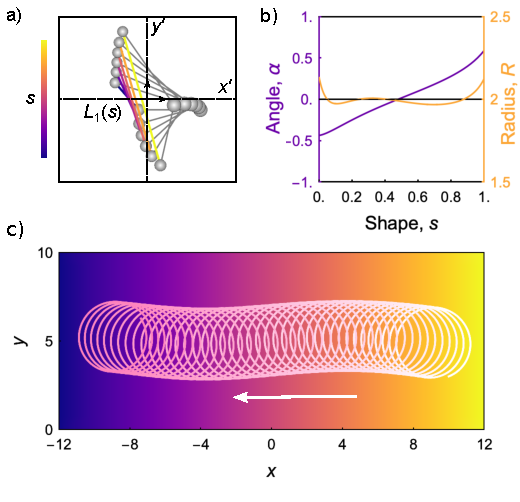
\includegraphics[width=9cm]{figures/A3_FigureS3.pdf}
    \caption{Design of a three-sphere cluster with a negative chemotactic response. (a) Standard shapes for the optimal design for different values of the shape parameter $s=(L_1-L_{\min})/(L_{\max}-L_{\min})\in [0,1]$. During optimization, we prescribe the lengths $L_3=0.6$, $L_{\min}=0.35$, $L_{\max}=1.35$ and $R_0=2$; the optimal design identified is $a_1=0.0562$, $a_2=0.0516$, $a_3=0.0683$, and $L_2=0.874$. (b) Computed response functions $\alpha(s)$ and $R(s)=U(s)/\Omega(s)$ for the standard shapes in (a). (c) Computed particle trajectory on a uniform stimulus gradient $S(\ve{x})=Gx$ of magnitude $G=0.2$; the shape parameter is assume to vary with the local stimulus as $s = (1+ e^{-S})^{-1}$.}
    \label{fig:negChemo}
\end{figure}

%%%%%%%%%%%%%%%%%%%%%%%%%%%%%%%%%%%%%%%%%
%%%%%%%%%%%%%%%%%%%%%%%%%%%%%%%%%%%%%%%%%
%%%%%%%%%%%%%%%%%%%%%%%%%%%%%%%%%%%%%%%%%
\clearpage
\section{Designed cluster moving perpendicular to the gradient}

To design clusters that move perpendicular to the gradient direction, we use a different objective function that characterizes the variations in the propulsion angle $\alpha$ about its mean value (which can be set to zero without loss of generality)
\begin{equation}
    O(\ve{d}) = \langle \alpha(s,\ve{d})^2 \rangle_s - \langle \alpha(s,\ve{d}) \rangle^2_s
\end{equation}
Moreover, we constrain the quantity $d R/d s$ to be positive or negative to control the direction of motion perpendicular to the gradient (Fig. \ref{fig:perpChemo}).

\begin{figure}[h]
    \centering
    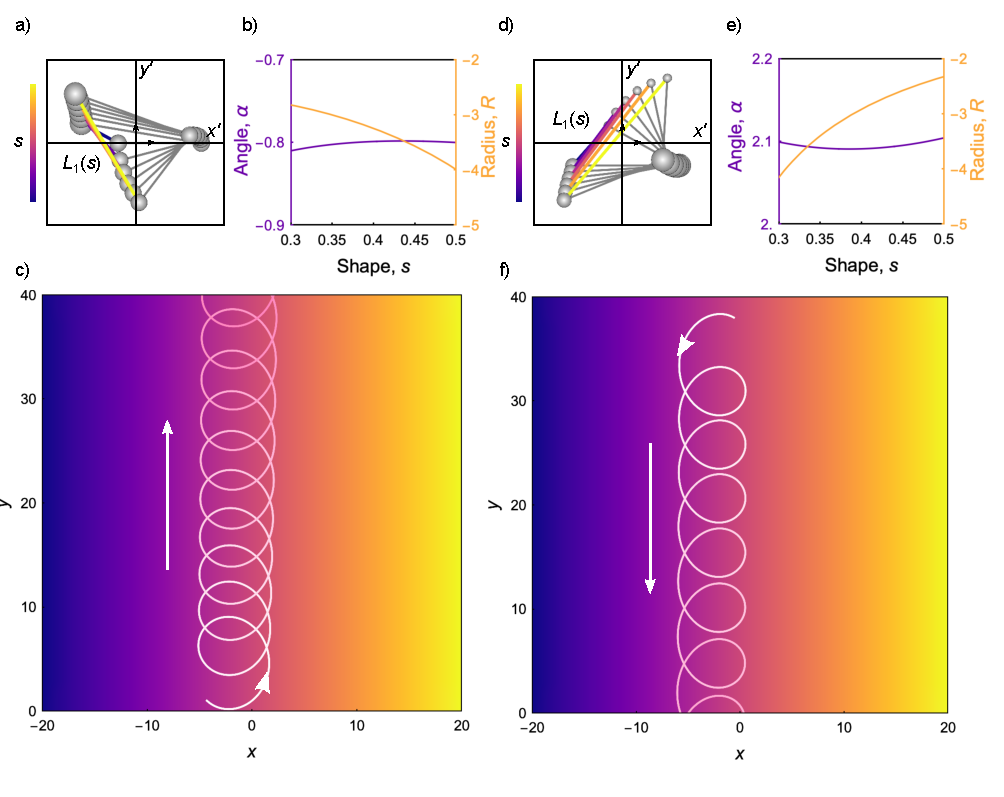
\includegraphics[width=15cm]{figures/A3_FigureS4.pdf}
    \caption{Design of two three-sphere clusters that move perpendicular to the stimulus gradient. (a,d) Standard shapes for the optimal design for different values of the shape parameter $s=(L_1-L_{\min})/(L_{\max}-L_{\min})\in [0,1]$.
    We prescribe the lengths as $L_3=1$, $L_{\min}=0.5$, $L_{\max}=1.5$. The optimal design identified for (a) is $a_1=0.1$, $a_2=0.135$, $a_3=0.1$, and $L_2=1.410$; the optimal design for (d) is $a_1=0.0670$, $a_2=0.040$, $a_3=0.108$, and $L_2=0.767$. (b,e) Computed response functions $\alpha(s)$ and $R(s)=U(s)/\Omega(s)$ for the standard shapes in (a) and (d). (e,f) Computed particle trajectory on a uniform stimulus gradient $S(\ve{x})=Gx$ of magnitude $G=0.2$; the shape parameter is assume to vary with the local stimulus as $s = (1+ e^{-S})^{-1}$.}
    \label{fig:perpChemo}
\end{figure}



%%%%%%%%%%%%%%%%%%%%%%%%%%%%%%%%%%%%%%%%%
%%%%%%%%%%%%%%%%%%%%%%%%%%%%%%%%%%%%%%%%%
%%%%%%%%%%%%%%%%%%%%%%%%%%%%%%%%%%%%%%%%%
\clearpage
\section{Derivation of the drift velocity with Brownian motion}

%%%%%%%%%%%%%%%%%%%%%%%%%%%%%%%%%%%%%%%%%
%%%%%%%%%%%%%%%%%%%%%%%%%%%%%%%%%%%%%%%%%
\subsection{Analytical solution of a simplified model}

To describe the effects of Brownian motion on the shape-directed dynamics of active particles, we introduce fluctuating forces, $F_x(t)$ and $F_y(t)$, and torque, $L(t)$, to the deterministic dynamics of equations (\ref{eq:theta}), (\ref{eq:xp}), and (\ref{eq:yp}) for the particle orientation $\theta$ and position $x,y$
\begin{align}
    \dot{\theta} &= \Omega + \frac{1}{\xi_r}L(t) \label{eq:langevin1}
    \\ 
    \dot{x} &= U \cos(\theta + \alpha)  + \frac{1}{\xi}F_x(t)  
    \\ 
    \dot{y} &= U \sin(\theta + \alpha) + \frac{1}{\xi}F_y(t) \label{eq:langevin3}
\end{align}	
where $\xi_r$ and $\xi$ are friction coefficients for rotation and translation, respectively.  For simplicity, we neglect any frictional coupling between the three degrees of freedom.  The fluctuating forces and torque have zero mean and satisfy the fluctuation-dissipation relation
\begin{gather}
    \langle F_x(t) \rangle = 0 \quad \text{and} \quad \langle F_x(t)F_x(t') \rangle = 2\xi k_B T\delta(t,t')
    \\
    \langle F_y(t) \rangle = 0 \quad \text{and} \quad \langle F_y(t)F_y(t') \rangle = 2\xi k_B T\delta(t,t')
    \\
    \langle L(t) \rangle = 0 \quad \text{and} \quad \langle L(t)L(t') \rangle = 2\xi_r k_B T\delta(t,t')
\end{gather}
where $k_B T$ is the thermal energy.  These overdamped Langevin equations are more conveniently described by the corresponding Fokker-Planck equation for the distribution function $f(x,y,\theta,t)$
\begin{equation}
    \frac{\partial f}{\partial t} + \frac{\partial}{\partial \theta}(\Omega f) + \frac{\partial}{\partial x}\left[ U \cos(\theta+\alpha)f\right] + \frac{\partial}{\partial y}\left[ U \sin(\theta+\alpha)f\right] =  \frac{k_B T}{\xi_r}\frac{\partial^2f}{\partial \theta^2} + \frac{k_B T}{\xi} \left(\frac{\partial^2 f}{\partial x^2}+ \frac{\partial^2 f}{\partial y^2}\right)
\end{equation}

We consider the motion of a particle with the simple response functions, $U(S)=U$, $\Omega(S)=\Omega$, and  $\alpha(S)=S$, on a uniform stimulus gradient, $S=G x$, of magnitude $G$. For this problem, we can neglect variations in $y$ such that $f(x,y,\theta,t)=f(x,\theta,t)$.  Scaling lengths by $R=U/\Omega$ and time by $\Omega^{-1}$, the Fokker-Planck equation simplifies as
\begin{equation}
    \frac{\partial f}{\partial t} + \frac{\partial f}{\partial \theta} + \frac{\partial}{\partial x}\left[\cos(\theta+Gx)f\right] =  \frac{1}{\text{Pe}_r}\frac{\partial^2f}{\partial \theta^2} + \frac{1}{\text{Pe}}\frac{\partial^2 f}{\partial x^2}
\end{equation}
where $\text{Pe}_r = \Omega \xi_r/k_B T$ and $\text{Pe}=U R \xi/k_B T$ are P\'eclet numbers for rotation and translation, respectively.  This equation admits periodic solutions on the domain $0<\theta<2\pi$ and $0<x<2\pi/G$. At long times, the distribution function approaches the following solution valid for weak gradients
\begin{equation}
    f(x,\theta) \propto \frac{1 + \text{Pe}_r^2}{G\text{Pe}_r} - \text{Pe}_r \cos (\theta + G x) + \sin (\theta + G x) + \mathcal{O}(G)
\end{equation}
From this result, the drift velocity in the $x$ direction can be evaluated as 
\begin{equation}
    V = \frac{\int_0^{2\pi} \cos(\theta+G x)f(x,\theta) d\theta}{\int_0^{2\pi} f(x,\theta) d\theta} = -\frac{G \text{Pe}_r^2}{2 (1 + \text{Pe}_r^2)}  + \mathcal{O}(G^2)
\end{equation}
For high P\'eclet number ($\text{Pe}_r\gg1$), this result is identical to that of equation (\ref{eq:xdrift2}).  For low P\'eclet number ($\text{Pe}_r\ll 1$), the drift velocity scales as $V\sim -\tfrac{1}{2}G\text{Pe}_r^2$.

%%%%%%%%%%%%%%%%%%%%%%%%%%%%%%%%%%%%%%%%%
%%%%%%%%%%%%%%%%%%%%%%%%%%%%%%%%%%%%%%%%%
\subsection{Numerical solution of the Langevin equation}

To simulate particle motions with arbitrary response functions and stimulus landscapes, we also implemented numerical simulations of the following Langevin equation for translational and rotational motion,
\begin{equation}
    \ve{m}\cdot \frac{d\ve{\mathcal{U}}}{d t} = \ve{\mathcal{F}}_A + \ve{\mathcal{F}}_H + \ve{\mathcal{F}}_B \label{eq:langevin}
\end{equation}
where $\ve{m}$ is a generalized mass/moment-of-inertia tensor, $\ve{\mathcal{U}} = (\ve{U}, \ve{\Omega})$ is the particle translational/rotational velocity vector, $\ve{\mathcal{F}}_A =(\ve{F}_A, \ve{L}_A)$ is the activity induced force/torque vector, $\ve{\mathcal{F}}_H$ is the hydrodynamic force/torque vector, and $\ve{\mathcal{F}}_B$ is the stochastic force/torque that gives rise to Brownian motion.\autocite{Brady1988a}  At low Reynolds numbers, the hydrodynamic force on the particle is linearly related to its velocity as $\ve{\mathcal{F}}_H = -\ve{\mathcal{R}} \cdot\ve{\mathcal{U}}$, where $\ve{\mathcal{R}}$ is the hydrodynamic resistance tensor. Consistent with equations (\ref{eq:motion1}) and (\ref{eq:motion2}) for the self-phoretic velocity, the activity induced force is equal and opposite to the hydrodynamic force, $\ve{\mathcal{F}}_A = -\ve{\mathcal{F}}_H$. The stochastic force/torque $\ve{\mathcal{F}}_B$ arises from thermal fluctuations and is characterized by
\begin{equation}
    \langle \ve{\mathcal{F}}_B \rangle =0 \quad  \text{and} \quad \langle \ve{\mathcal{F}}_B(0)\ve{\mathcal{F}}_B(t)\rangle = 2 k_B T \ve{\mathcal{R}} \delta(t)
\end{equation}
where $k_B T$ is the thermal energy, the angle brackets denote an ensemble average, and $\delta(t)$ denotes the delta function.  In contrast to the simplified model of equations (\ref{eq:langevin1})-(\ref{eq:langevin3}), this formulation accounts for the shape-dependent coupling between particle translation and rotation, which arise due to non-zero off-diagonal elements in the resistance tensor $\ve{\mathcal{R}}$. The Langevin equation (\ref{eq:langevin}) was integrated numerically in the overdamped regime, using Fixman’s midpoint scheme with a constant time step of $\Delta t = 500$ (in units of $L D/\mu A$), which is small relative to the time $L/U\sim 10^4$ based on the computed velocity.\autocite{delmotte2015simulating,Delong2015}  Figure \ref{fig:noise} illustrates two stochastic particle trajectories showing particle chemotaxis in the presence of Brownian motion.

\begin{figure}[h]
    \centering
    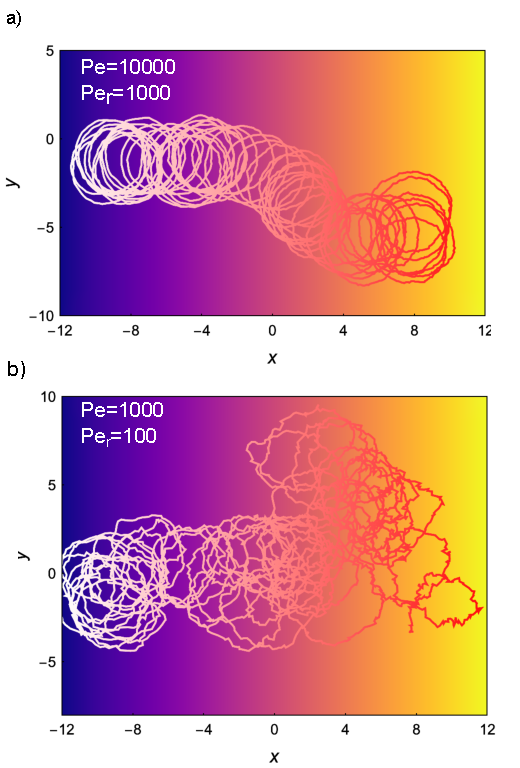
\includegraphics{figures/A3_FigureS5.pdf}
    \caption{Noisy trajectories on a uniform stimulus gradient $S(\ve{x})=Gx$ of magnitude $G=0.2$ for particles with the same geometry and shape-shifting response as those in Figure 3 of the main text: sphere radii $a_1=0.1$, $a_2=0.0985$, and $a_3=0.0958$; bond lengths $L_1\in[0.5,1.5]$, $L_2=0.677$, $L_3=1$. The magnitude of the noise is characterized by the rotational P\'eclet number, $\text{Pe}_r = \Omega \xi_r/k_B T$, using the computed value of $\xi_r$ for $s=0.5$.  The shape parameter is assume to vary with the local stimulus as $s = (1+ e^{-S})^{-1}$.}
    \label{fig:noise}
\end{figure}


                     
                  




\end{appendices}